\documentclass[11pt,final]{article}
\usepackage{a4wide}
\usepackage{color}
\usepackage{graphicx}
\usepackage{listings}
\usepackage{hyperref}
\usepackage{array}
\usepackage{xspace}
\usepackage{comment}

\setlength{\parindent}{0pt}
\setlength{\parskip}{5pt}

\definecolor{lightgray}{rgb}{.95,.95,.95}

\lstset{
  language=bash,
  backgroundcolor=\color{lightgray}
}

\newcommand{\Gt}[0]{\emph{GenomeTools}\xspace}
\newcommand{\Gtj}[0]{\emph{GenomeTools-Java}\xspace}
\newcommand{\FO}[0]{\emph{FISH Oracle}\xspace}


\title{The \FO user manual}
\author{Malte Mader}

\begin{document}

\maketitle
\tableofcontents

\section{Introduction}

This user manual describes how to install, configure and maintain the
\FO software. To get a first impression of the software visit 
\url{http://ww.zbh.uni-hamburg.de/fishoracle} to watch the screencast or
try out the demo server. 
\begin{comment}
We also offer a virtual machine with an 
already set up \FO application which provides a quick and easy way to 
use a private instance of \FO. If you want to use FISH Oracle 
collaboratively in production mode we encourage to set up a private
installation at an own machine. Due to the technical limitations of 
virtual machines (slow, little storage) its use for large amounts of 
data is not recommendable.
\end{comment}

\section{Installation}

\subsection{Requirements and Availability}

To be able to install FISH Oracle the following software packages are needed:

\begin{itemize}
  \item MySQL server
  \item Apache Tomcat server
  \item \Gt
  \item \FO
\end{itemize}

If you want to install Apache or MySQL manually you can download it from
\url{http://tomcat.apache.org/} and \url{http://www.mysql.com/downloads/mysql/}
respectively. This is only necessary if you do not have administration rights
on the system you want to install the \FO.
\Gt is available for download from \url{http://genometools.org/pub/}.
\Gtj and \FO can be obtained from \url{http://www.zbh.uni-hamburg.de/fishoracle}.

\subsection{Installation on Linux Distributions}

\subsubsection{Debian 6.0}

An installation script for the automatic installation of all needed software
packages and the FISH Oracle software is provided at
\url{http://www.zbh.uni-hamburg.de/fileadmin/gi/FISHOracle/install_fishoracle_debian.sh}.
The script needs to be executed with administration rights.

If you want to install the needed software manually open a terminal.
If you have installed the gnome Desktop open a terminal with:
Applications$\rightarrow$Accessories$\rightarrow$Terminal and execute the 
following commands as administrator:

\begin{lstlisting}
 > echo deb http://ftp.de.debian.org/debian squeeze main \
   contrib non-free >> /etc/apt/sources.list

 > apt-get update

 > apt-get install mysql-server sun-java6-jdk

 > echo 'JAVA_HOME="/usr/lib/jvm/java-6-sun"' >> /etc/environment
 > echo 'JRE_HOME="/usr/lib/jvm/java-6-sun/jre"' >> /etc/environment

 > export JAVA_HOME="/usr/lib/jvm/java-6-sun"

 > apt-get install ant tomcat6 libcairo2-dev libncurses5-dev
\end{lstlisting}

\subsubsection{Ubuntu 10.10}

An installation script for the automatic installation of all needed software
packages and the FISH Oracle software is provided at
\url{http://www.zbh.uni-hamburg.de/fileadmin/gi/FISHOracle/install_fishoracle_ubuntu.sh}.
The script needs to be executed with administration rights

Open a terminal: Applications$\rightarrow$Accessories$\rightarrow$Terminal and execute the 
following commands:

\begin{lstlisting}
 > sudo add-apt-repository ppa:sun-java-community-team/sun-java6

 > sudo apt-get update

 > sudo apt-get install mysql-server sun-java6-jdk ant tomcat \
   libcairo2-dev libncurses5-dev
\end{lstlisting}

%\subsubsection{OpenSUSE Linux 11.4}

\subsubsection{Installation of FISH Oracle specific software}

The last part of the installation is distribution independent
and therefore at every system the same. If the PC is a 64 bit
architecture the \Gt need to be compiled with the 64bit
flag \textit{make 64bit=yes}, otherwise only \textit{maker}.

\begin{lstlisting}
 > wget http://genometools.org/pub/genometools-1.3.7.tar.gz

 > tar -xvzf genometools-1.3.7.tar.gz

 > cd genometools-1.3.7

 > make

 > sudo make install

 > wget http://www.zbh.uni-hamburg.de/fileadmin/gi/ \
   FISHOracle/fishoracle.tar.gz

 > tar -xvzf fishoracle.tar.gz

 > cd fishoracle
\end{lstlisting}

Before compiling the FISH Oracle application, the database connections have 
to be set up. The databases installation is explained in the next chapter.
The connections are specified in 
\textit{war/config/database.conf}. The configuration parameters need to be 
adapted to your database names and login specifications. The structure of the
file looks as follows:

\begin{verbatim}

[ensembl]

host = localhost
port = 3306
db = ensembl
user = mysql_user
pw = mysql_password

[fishoracle]

host = localhost
db = fishoracle
user = mysql_user
pw = mysql_password

\end{verbatim}

Finally the application can be compiled and copied to the Tomcat server:

\begin{lstlisting}
 > ant war 

 > cp fishoracle.war /var/lib/tomcat6/webapps
\end{lstlisting}

Now the FISH Oracle application should be accessible at 
\url{http://localhost:8080/fishoracle}. Last but not least the databases
need to be installed to be able to use FISH Oracle.

\subsection{Databases}

\paragraph{Ensembl database.}

Download the genome of your choice from 
\url{ftp://ftp.ensembl.org/pub/current/mysql/}.

If you want to download e.g. the human genome execut the following command
in the console:

\begin{lstlisting}
 > wget r ftp://ftp.ensembl.org/pub/current/mysql/ \
        homo_sapiens_core_61_37f/*.gz
\end{lstlisting}

Create a database, unpack all tar files and import the SQL schema and data
into the database:

\begin{lstlisting}
 > mysql -u db_user -p

 mysql> CREATE DATABASE ensembl;

 > mysql -u db_user -p ensembl < homo_sapiens_\
   core_61_37f.sql

 > mysqlimport -u db_user -p --fields_escaped_by=\\ \
   homo_sapiens_core_61_37f -L *.txt
\end{lstlisting}

\paragraph{FISH Oracle database.}

Create a FISH Oracle database. Download the FISH Oracle source code if you 
have not done so already and import the SQL database schema plus initial
data into
the FISH Oracle database:


\begin{lstlisting}
 > wget http://www.zbh.uni-hamburg.de/fishoracle/fishoracle.tar.gz
 > tar -xvzf fishoracle.tar.gz
 mysql> CREATE DATABASE fishoracle;
 mysql> USE fishoracle;
 mysql> SOURCE fishoracle.sql;
\end{lstlisting}

\subsection{Setup initial user}

In the last installation step an initial user with administration rights 
should be created. Open your browser, load the FISH Oracle application
and register this user.

Next, open a terminal and login to the MySQL console and type the following 
commands:

\begin{lstlisting}
 mysql> use fishoracle;
 mysql> update user set isactive = 1;
 mysql> update user set isadmin = 1;
\end{lstlisting}

Now you can use FISH Oracle.

%\subsection{Install \Gt from source}

%\subsection{Install \Gtj from source}

%\subsection{Install Java manually}

%\subsection{Install Tomcat manually}

\section{Configuration}

\subsection{Data Import}

New data is imported from tab delimited files. The data format of these files needs to
include the following data columns:

\begin{enumerate}
  \item Row count column (header row stays empty)
  \item ID column (``ID'')
  \item Chromosome column (``chr'')
  \item Start position (``start'')
  \item End position (``end loc'')
  \item Number of markers (``markers'')
  \item Segment mean intensity value (``segment mean'')
\end{enumerate}

Table \ref{tab:tsv} exemplifies the structure of a tab delimited import file.

\begin{table}
	\centering
	\begin{tabular}[h]{|c|c|c|c|c|c|c|}
	  \hline
	  & ID & chr & start & end loc & markers & segment mean \\ \hline
	 1 & pancreas\_experiment001 & 1 & 10000 & 20000 & 135 & -0.27 \\
	 2 & pancreas\_experiment001 & 1 & 21000 & 25000 & 57 & 0.01 \\
	 3 & pancreas\_experiment001 & 1 & 25001 & 30000 & 80 & -0.3 \\
	 4 & pancreas\_experiment001 & 2 & 3000 & 5000 & 22 & 0.21 \\
	 5 & pancreas\_experiment001 & 2 & 8000 & 10000 & 15 & 0.28 \\
	 6 & pancreas\_experiment001 & 2 & 11000 & 18000 & 47 & 0.3 \\
	 \vdots & \vdots & \vdots & \vdots & \vdots & \vdots & \vdots \\
	\end{tabular}
	\caption{Structure of the tab delimited import files.}
	\label{tab:tsv}
\end{table}

The data import comprises 2 steps: The upload of the tab delimited file and 
the actual import of the data and meta data into the database.
After the upload the user needs to specify an appropriate microarray study
name. By default the file name is suggested. Furthermore the chip type and a 
tissue need to be specified. Figure \ref{fig:import} depicts the data import.

\begin{figure}[h]
	\begin{center}
	  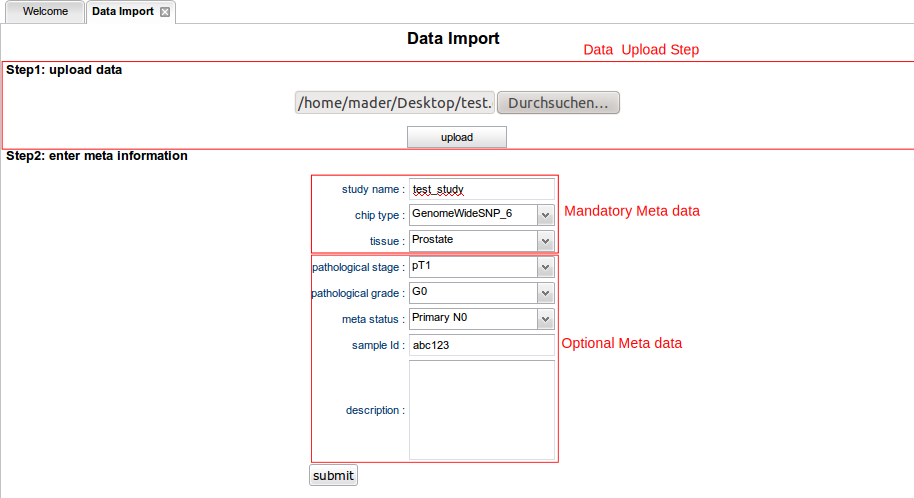
\includegraphics[width=\textwidth]{fig/import.pdf}
	\end{center}
	\caption{Screenshot of the import page.}
	\label{fig:import}
\end{figure}

%\subsection{Run more than one \FO-Application on a Tomcat server}

\subsection{Database Connection}

The database connection can either be configured directly in the configuration
file in \textit{webapps/fishoracle/war/config/database.conf} under the 
Tomcat main directory or directly in the web application.
The changes take effect immediately after saving the changes in the file or
submitting the changes via the application. There is no need to restart the 
Tomcat server or to recompile the application. Figure \ref{fig:dbconfig} illustrates 
the database configuration interface.

\begin{figure}[h]
	\begin{center}
		\includegraphics[width=\textwidth]{fig/dbconfig.png}
	\end{center}
	\caption{The database configuration interface provides the possibility
	         to change the database connection instantly.}
	\label{fig:dbconfig}
\end{figure}

\subsection{AnnotationSketch Visualization}

The appearance of the visualizations can be influenced by a configuration file
located in \textit{war/config/default.style}. The file contains Lua code that 
is used in the rendering process of the images. It includes display 
definitions for genes, segment data, various genomic and non-genomic elements
as well as global display options corresponding to the spacing or visibility 
of elements and captions. For detailed explanation of the style file see 
\url{http://genometools.org/style_options.html}. 

This section mentions the most important options to customize the 
visualization of FISH Oracle.

The options for the display of segment data e.g. looks as follows:
\begin{verbatim}

cnc = {
    -- Color definitions
    stroke_marked      = {red=1.0, green=0.0, blue=0.0},
    style              = "box",
  }, 

\end{verbatim}

The option \textit{stroked\_marked} means in this example, that a found element
representing segment data will be marked with a red border. The option 
\textit{style} determines that all elements will be drawn as a rectangular
box.

To get a more compact visualization captions of elements could be disabled
and spaces between tracks could be adapted:

\begin{verbatim}

show_block_captions = false, -- generally show captions
show_track_captions = false, -- generally show track captions

bar_vspace = 5,   -- space between feature bars, in pixels
track_vspace = 15, -- space between tracks, in pixels

\end{verbatim}

The display of captions for specific elements is also adjustable with the
\textit{max\_capt\_show\_width} option. The value is a threshold up to which
captions are shown. If the width of the displayed sequence region 
(in characters) exceeds this value, then captions are omitted. If set to 0,
captions are never shown for this type. If set to \textit{nil}, then captions are
always shown (\url{http://genometools.org/style_options.html}).  
The following example shows the option in the context of segment data where 
captions are completely disabled.

\begin{verbatim}

cnc = {
    -- Color definitions
    stroke_marked      = {red=1.0, green=0.0, blue=0.0},
    style              = "box",
    max_capt_show_width= 0,
  }, 


\end{verbatim}

%\section{Usage}

\end{document}
